\section{ANSI-Escapesequenzen}
\label{sec:referenz:ansi-esc}

Die ANSI-Escapesequenzen (oder auch ANSI-Escapecodes) 
\begin{marginfigure}%
    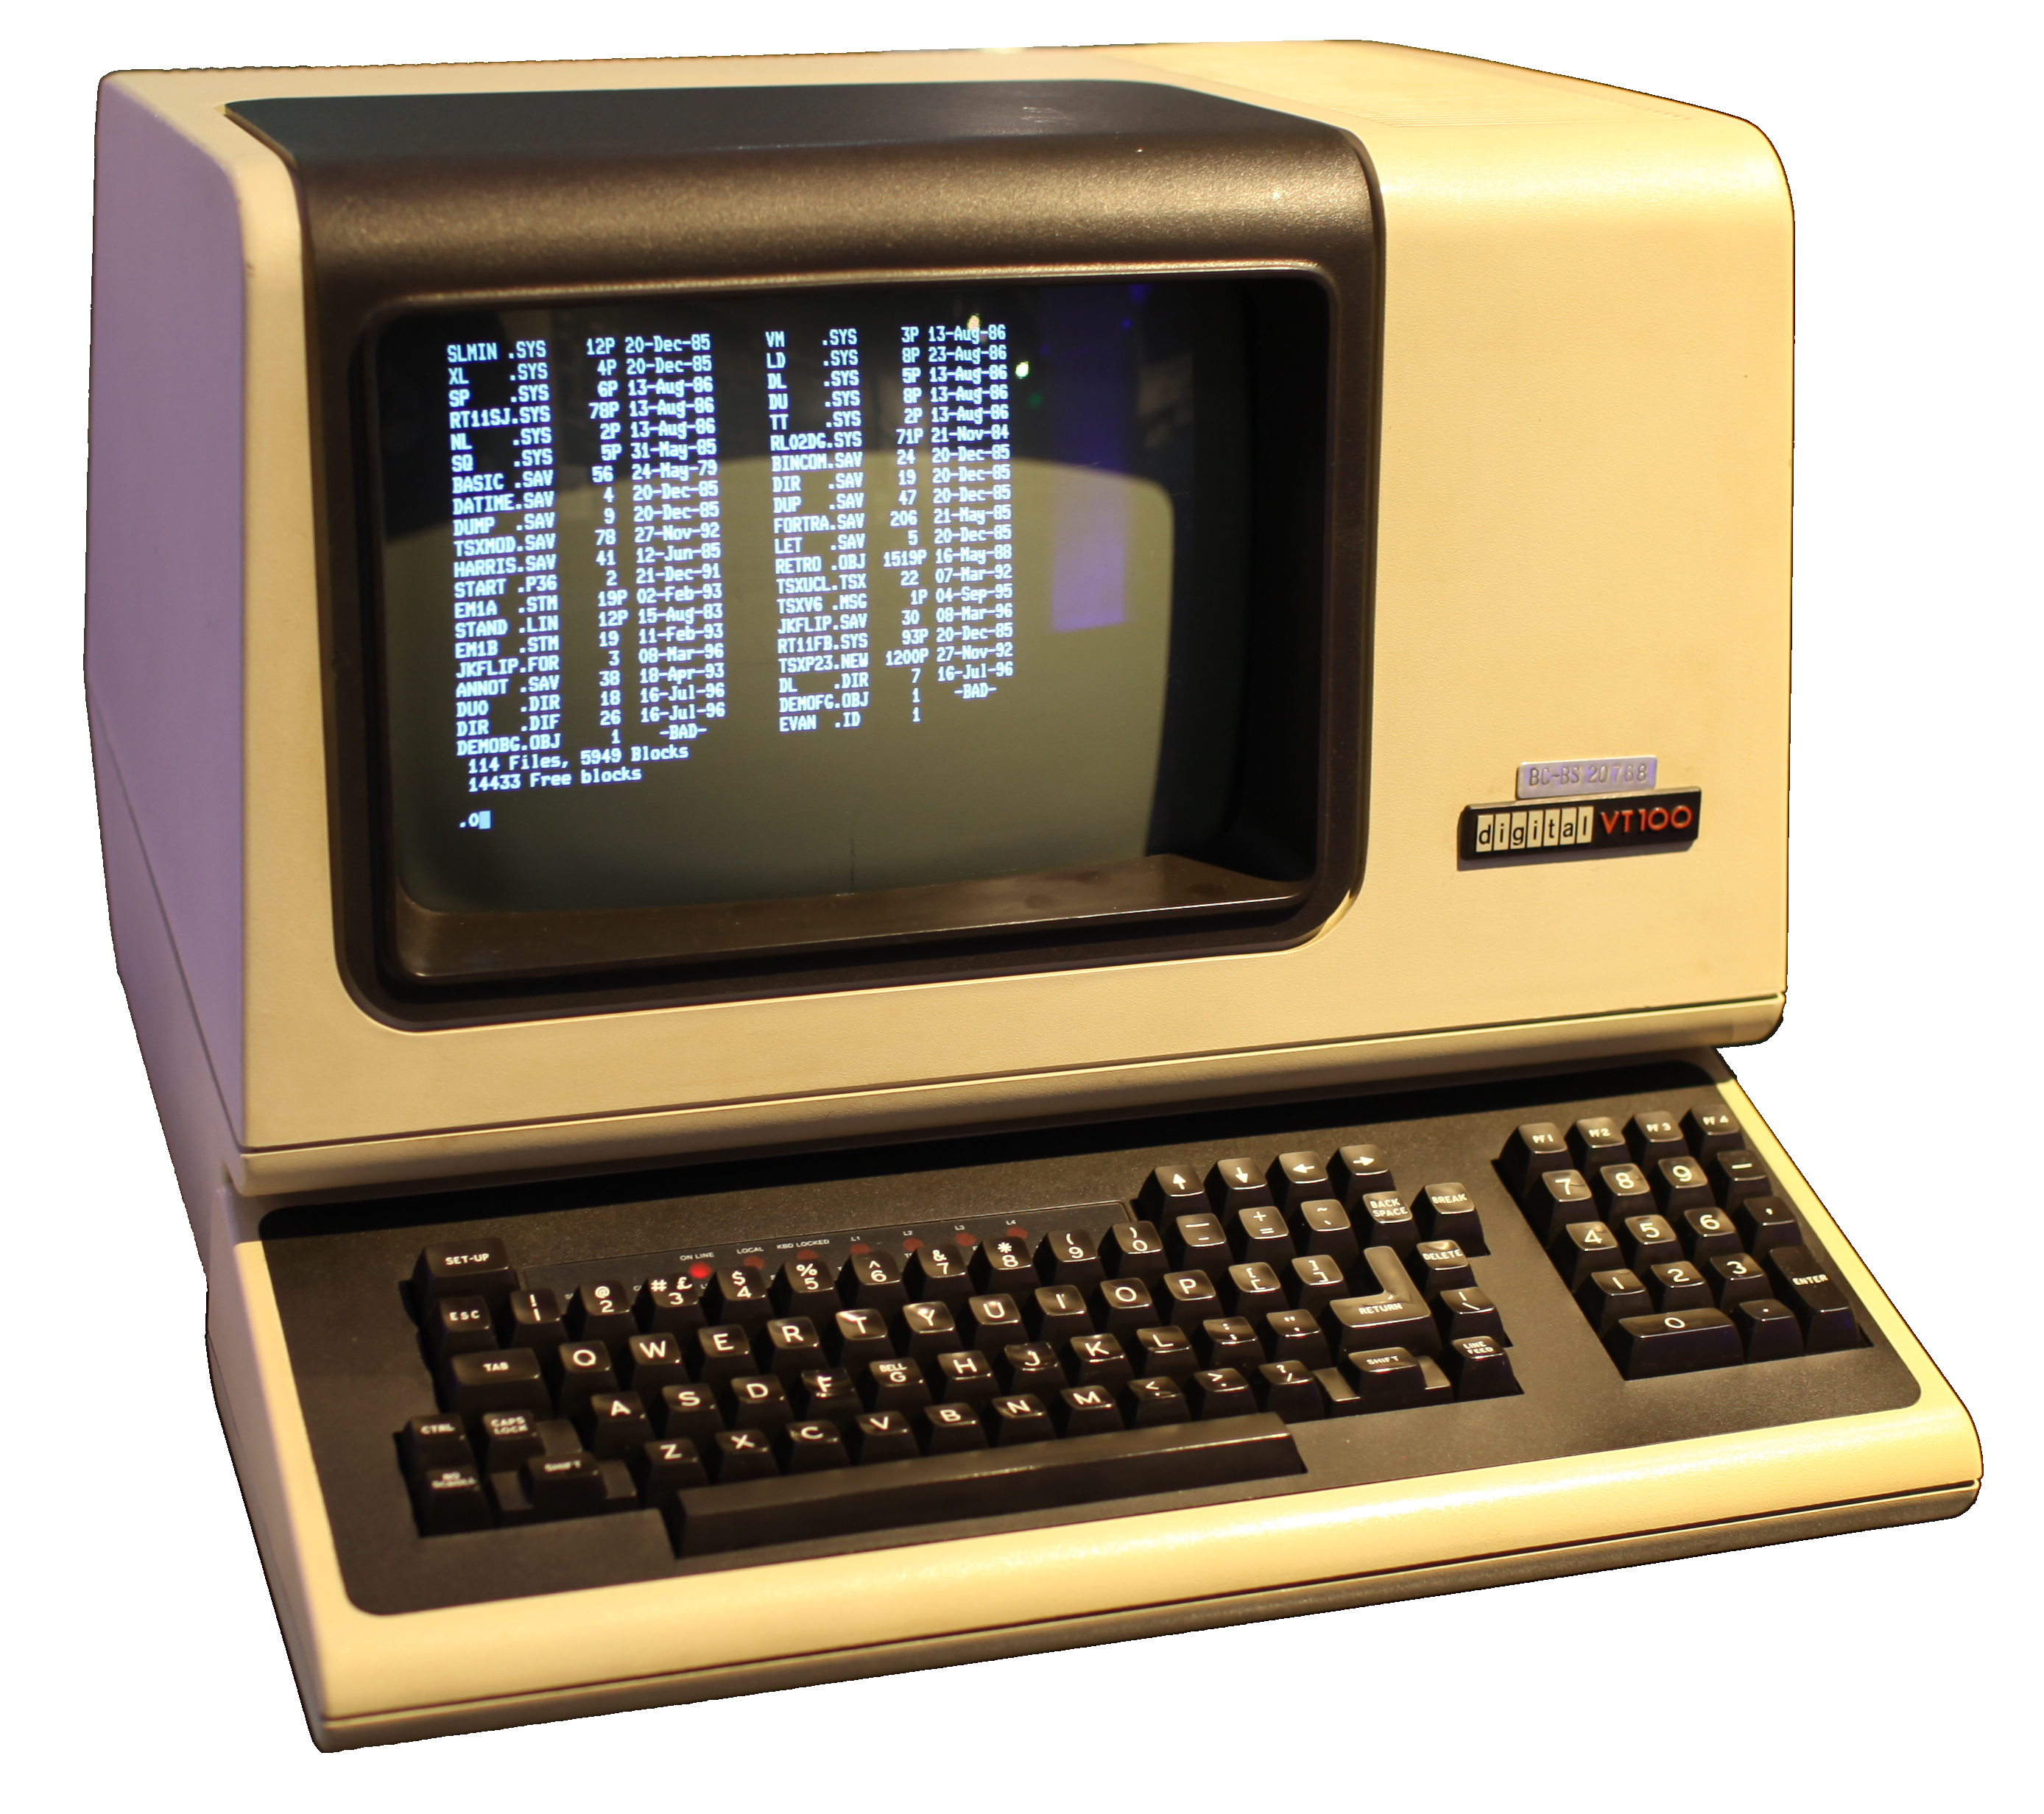
\includegraphics[width=\linewidth]{images/DEC_VT100_terminal_transparent.png}
    \caption{Der VT100 von Digital Equipment Corporation (DEC), gebaut von 1978 bis 1983. (Foto: Gorthmog, \href{https://creativecommons.org/licenses/by-sa/4.0}{CC BY-SA 4.0}, via Wikimedia Commons)}%
    \label{fig:referenz:vt100}
\end{marginfigure}
wurden nicht für moderne Computer erfunden, sondern für Terminals — Bildschirme, die aussahen wie ein Fernseher mit Tastatur und die über eine Leitung mit einem großen Computer verbunden waren. Einer der bekanntesten war der VT100 (siehe Abbildung) von Digital Equipment Corporation (DEC). Auf seinem Bildschirm gab es 24 Zeilen mit je 80 Zeichen — und der Cursor war ein echter, sichtbarer Block, der auf dem Bildschirm stand. Die ANSI-Escapesequenzen, die Ihr heute benutzt, sind die Sprache, mit der man diesen Cursor und den Bildschirm steuert. Moderne Terminals (wie die Konsole auf Eurem Raspberry Pi) verstehen dieselben Sequenzen — sie sind sozusagen die ‚Muttersprache' der Konsole.

Die wichtigsten Sequenzen sind die sogenannten CSI\footnote{%
    CSI steht für ``Control Sequence Introducer'', was so viel wie ``Kontrollsequenzeinführung'' auf deutsch bedeutet.}
Sequenzen -- das CSI steht für \esc{x1B[}, darauf folgen eventuell verschiedene Parameterzeichen (siehe unten) und schließen mit einem Buchstaben, sozusagen dem Kommandocode, ab. 
Ein Beispiel dazu ist \texttt{"\textbackslash x1B[H"}, das Ihr in der Funktion \codeinline{konsole_start} kennengelernt habt. Dabei steht \texttt{H} für das setzen der Cursorposition. Wenn Ihr nun denkt, dann müsste man ja auch die Zeile und Spalte angeben können -- Ihr habt recht, das geht folgendermaßen: \codeinline{printf("\x1B[\%d;\%dH", zeile, spalte);}
Wenn man die Zahlen weglässt, werden also Standardwerte verwendet, in diesem Fall jeweils für Zeile und Spalte die 1.

Es gibt eine ganze Menge an CSI-Sequenzen. Die, die wir in den Beispielen, Programmen, und Übungen verwenden werden -- und auch ein paar mehr, mit denen Ihr vielleicht spielen wollt, zum Beispiel den Farben, sind in den folgenden Tabellen aufgelistet:

\begin{table*}[h]
  \begin{tabular}{cclp{8cm}}
    \toprule
    \textbf{CSI} & \textbf{printf} & \textbf{Name} & \textbf{Effekt} \\
    \midrule
    \texttt{CSI n A}        & \texttt{"\textbackslash x1B[\%dA"}         & Cursor nach oben & 
        Bewegt den Cursor \texttt{n} (Standard ist \texttt{1}) mal nach oben. \\ 
    \texttt{CSI n B}        & \texttt{"\textbackslash x1B[\%dB"}         & Cursor nach unten & 
        Bewegt den Cursor \texttt{n} (Standard ist \texttt{1}) mal nach unten. \\ 
    \texttt{CSI n C}        & \texttt{"\textbackslash x1B[\%dC"}         & Cursor nach rechts & 
        Bewegt den Cursor \texttt{n} (Standard ist \texttt{1}) mal nach rechts. \\ 
    \texttt{CSI n D}        & \texttt{"\textbackslash x1B[\%dD"}         & Cursor nach links & 
        Bewegt den Cursor \texttt{n} (Standard ist \texttt{1}) mal nach links. \\ 
    \texttt{CSI n ; m H}    & \texttt{"\textbackslash x1B[\%d;\%dH"}     & Cursorposition & 
        Bewegt den Cursor in Zeile \texttt{n} und Spalte \texttt{m}. Zeile und Spalte beginnen bei 1, was auch der Standardwert ist, wenn die Zahlen weggelassen werden. \\
    \texttt{CSI n J}        & \texttt{"\textbackslash x1B[\%dJ"}        & Anzeige löschen &
        Löscht Zeichen auf der Konsole: \texttt{0} oder \texttt{1} löschen ab der Cursor-Position alles bis Konsolenende beziehungsweise -anfang. Die \texttt{2} löscht den gesamten Inhalt. \\ 
    \midrule
    \texttt{CSI n m}        & \texttt{"\textbackslash x1B[\%dm"}        & Grafikdarstellung &
        Wählt die Darstellung der Grafik aus. Ist \texttt{n} eine \texttt{0} oder wird weggelassen, werden alle Darstellungsoptionen zurückgesetzt. \\
    \bottomrule
  \end{tabular}
  \caption{Übersicht der ANSI-Escapesequenzen für die Cursor- und Grafiksteuerung.}
  \label{tab:referenz::ansi-esc}
\end{table*}

\newpage\noindent
Außerdem verwenden wir weitere Steuerungscodes, die nicht zum Standard gehören:
\begin{table*}[h]
  \begin{tabular}{cclp{8cm}}
    \toprule
    \textbf{CSI} & \textbf{printf} & \textbf{Name} & \textbf{Effekt} \\
    \midrule
    \texttt{CSI ? 25 h}        & \texttt{"\textbackslash x1B[?25h"}         & Cursor zeigen  & 
        Zeigt den Eingabecursor. \\ 
    \texttt{CSI ? 25 l}        & \texttt{"\textbackslash x1B[?25l"}         & Cursor verstecken &
        Versteckt den Eingabecursor. \\
    \bottomrule
  \end{tabular}
  \caption{Zusätzliche ANSI-Escapesequenzen für die Cursorsteuerung. Diese Sequenzen funktionieren auf fast allen modernen Terminals gehören aber nicht zum ursprünglichen ANSI-Standard.}
  \label{tab:referenz::ansi-esc:extra}
\end{table*}


\vskip5em
\paragraph{Darstellungsoptionen}

\begin{table}[h]
  \centering
  \begin{tabular}{cll}
    \toprule
    \textbf{n} & \textbf{Name} & \textbf{Hinweise} \\
    \midrule
    0 & Normal          & Setzt alle grafischen Optionen zurück. \\
    1 & Fettdruck       & \textbf{Ausgabe mit Fettdruck.} \\
    2 & Gedimmt         & \textcolor{gray}{Verringert die Helligkeit der Schrift.} \\
    3 & Kursiv          & \textit{Kursive (das heißt schräge) Schrift.} \\
    4 & Unterstreichung & \underline{Unterstreichung der Ausgabe.} \\
    7 & Invertierung    & \colorbox{black}{\textcolor{white}{Tauscht die Farben von Vorder- und Hintergrund.}} \\
    30--37 & Vordergrundfarbe & Setzen der Vordergrundfarbe (siehe Tab.~\ref{tab:referenz::ansi-esc:farben}). \\ 
    40--47 & Hintergrundfarbe & Setzen der Hintergrundfarbe. \\
    \bottomrule
  \end{tabular}
  \caption{Liste gebräuchlicher Darstellungsoptionen.}
  \label{tab:referenz::ansi-esc:grafik}
\end{table}

\paragraph{Farben}

\begin{table}[h]
  \centering
  \begin{tabular}{ccc}
    \toprule
    \textbf{Vordergrund} & \textbf{Hintergrund} & \textbf{Farbe (VGA)} \\
    \midrule
    30 & 40 & \cellcolor[RGB]{0,0,0}\textcolor{white}{Schwarz} \\
    31 & 41 & \cellcolor[RGB]{196,0,0}\textcolor{white}{Rot} \\
    32 & 42 & \cellcolor[RGB]{0,196,0}\textcolor{black}{Grün} \\
    33 & 43 & \cellcolor[RGB]{196,126,0}\textcolor{black}{Gelb} \\
    34 & 44 & \cellcolor[RGB]{0,0,196}\textcolor{white}{Blau} \\
    35 & 45 & \cellcolor[RGB]{196,0,196}\textcolor{white}{Magenta} \\
    36 & 46 & \cellcolor[RGB]{0,196,196}\textcolor{black}{Cyan} \\
    37 & 47 & \cellcolor[RGB]{196,196,196}\textcolor{black}{Weiß} \\
    \bottomrule
  \end{tabular}
  \caption{Die klassischen 8 Farben (VGA-Palette).}
  \label{tab:referenz::ansi-esc:farben}
\end{table}